\documentclass{standalone}
\usepackage{tikz}
\usepackage{amsmath}
\usetikzlibrary{positioning}

\tikzset{main node/.style={circle,,draw,minimum size=1cm,inner sep=0pt} }
\begin{document}

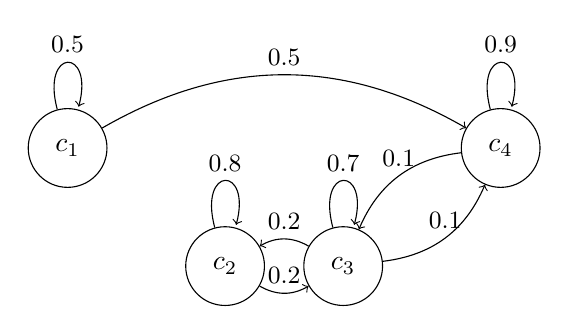
\begin{tikzpicture}
\begin{scope}[on grid]

  \node[main node] (1) {$c_1$};
  \node[main node] (2) [below right =1.5cm and 2cm of 1] {$c_2$};
  \node[main node] (3) [right =1.5cm of 2] {$c_3$};
  \node[main node] (4) [above right =1.5cm  and 2cm of 3] {$c_4$};

    \path[every node/.style={font=\sffamily\small}]
    (1) edge [loop above] node[above] {$0.5$}(1) 
    (2) edge [->, loop above] node[above] {$0.8$}(2)
    (3) edge [->, loop above] node[above] {$0.7$}(3)
    (4) edge [->, loop above] node[above] {$0.9$}(4)
    
    (1) edge [->, bend left ] node[above] {$0.5$}(4)
    (2) edge [->, bend right] node[above] {$0.2$}(3)
    (3) edge [->, bend right] node[above] {$0.2$}(2)
    (3) edge [->, bend right] node[above] {$0.1$}(4)
    (4) edge [->, bend right] node[above] {$0.1$}(3)

    ;
    \end{scope}
\end{tikzpicture}
\end{document}